\documentclass[12pt]{article}
% Эта строка — комментарий, она не будет показана в выходном файле
\usepackage{ucs}
\usepackage[warn]{mathtext}
\usepackage[utf8x]{inputenc} % Включаем поддержку UTF8
\usepackage[russian]{babel}  % Включаем пакет для поддержки русского языка
\usepackage{amsmath}
\usepackage{mathtools}
\usepackage{amssymb}
% \usepackage[dvips]{graphicx}
% \graphicspath{{noiseimages/}}
\usepackage[pdftex]{graphicx}


% Параметры страницы: 1см от правого края и 2см от остальных.


\hoffset=0mm
\voffset=0mm
\textwidth=180mm        % ширина текста
\oddsidemargin=-6.5mm   % левое поле 25.4 - 5.4 = 20 мм
\textheight=240mm       % высота текста 297 (A4) - 40
\topmargin=-15.4mm      % верхнее поле (10мм)
\headheight=5mm      % место для колонтитула
\headsep=5mm          % отступ после колонтитула
\footskip=8mm         % отступ до нижнего колонтитула

\begin{document}
	\author {Жарков Андрей 495}
	\title {Лабораторная работа 5.2 \\  Эффект Комптона.}
    \maketitle{}
    
    \begin{center}
    	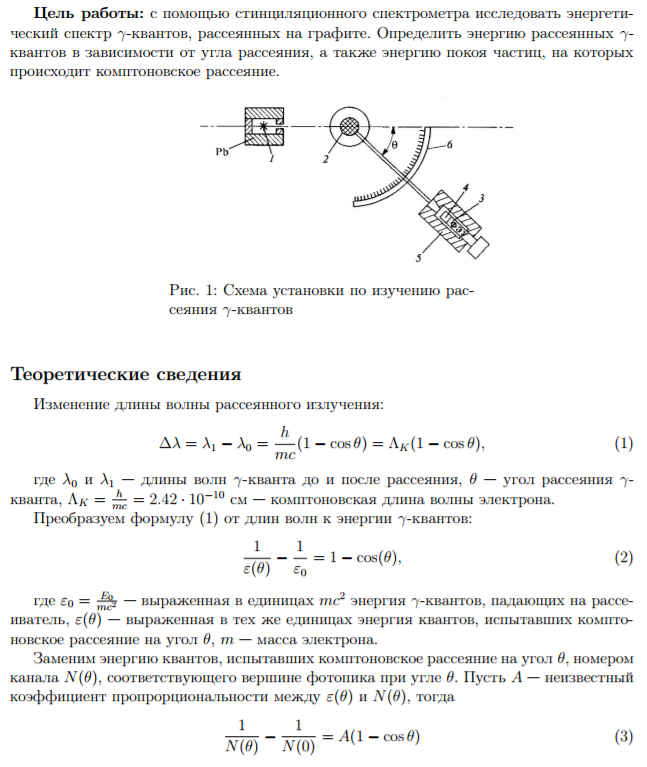
\includegraphics[width=15cm]{theory1.png}\\
    \end{center}
    
    \begin{center}
    	\textbf{\large Ход работы.}
    \end{center}
    
    1. Будем устанавливать сцинтилляционный счетчик под разными углами $\theta$ к первоначальному направлению полета $\gamma$-квантов. Снимем амплитудные спектры и определим положения фотопиков для каждого значения угла $\theta$. Результаты измерений приведены в таблице:\\
    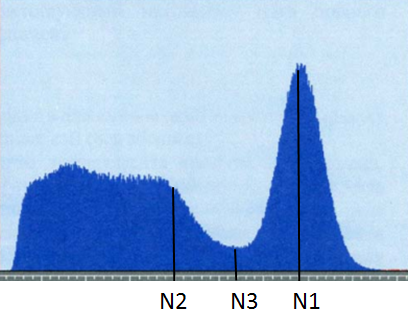
\includegraphics[width=8cm]{img.png}\\
    
\end{document}